\documentclass[conference]{IEEEtran}
\usepackage{biblatex}
\usepackage{graphicx}
\usepackage{amsmath}
\usepackage[spanish, english]{babel}
\usepackage{hyperref}
\usepackage{float}
\addbibresource{binomio.bib}
\def\BibTeX{{\rm B\kern-.05em{\sc i\kern-.025em b}\kern-.08em
    T\kern-.1667em\lower.7ex\hbox{E}\kern-.125emX}}
\begin{document}

\title{Complejidad ciclomática\\
{\footnotesize \textsuperscript{}Ciencias de la computación}
}

\author{\IEEEauthorblockN{Vicente Ferrari}
\IEEEauthorblockA{\textit{Dpto. de Cs. de la computación e Informática} \\
\textit{Universidad de la Frontera}\\
Temuco, Chile \\
v.ferrari01@ufromail.cl}

}


\maketitle

\selectlanguage{spanish}
\begin{abstract}
En este texto se explorará la complejidad ciclomática de un programa de reducción de laberintos.
\end{abstract}

\section{Introducción}

Los algoritmos se pueden visualizar como grafos de control de flujo. Esto da paso a una métrica en informática conocida como complejidad ciclomática. Como se observa en la Figura \ref{fig:control_flujo}.

\begin{figure}[H]
	\center{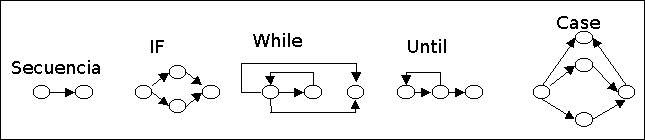
\includegraphics[scale=0.6]
	{control_flujo.png}}
	\caption{\label{fig:control_flujo} Grafos para las distintas estructuras de control.}
\end{figure}

\printbibliography


\end{document}
